\section{Inleiding}
\begin{styleframe}
        \frametitle{Inleiding}
Dit praatje is niet om te beschrijven hoe DNS technisch (op unix systemen) ge\"implementeerd is.

Hoewel dit onvermijdelijk is ligt de nadruk op een uitleg van DNS zonder ons (al te) druk te maken over de technische implementatie.
\end{styleframe}

\subsection{DNS?}
\begin{styleframe}
	\frametitle{DNS?}
\begin{itemize}
	\item DNS = Domain Name System.
	\item[] Grootste gedistrubueerde database ter wereld?
	\pause
\end{itemize}
Voornamelijk voor:
\begin{itemize}
	\item Hostnaam naar IP-adres vertaling (en andersom).
	\item[] {\bf Mensen zijn goed in namen (strings), computers goed in nummers}.
	\item[] Naam {\tt <->} nummer vertaling kom je vaker tegen, bv:
	\begin{itemize}
		\item username {\tt <->} uid
		\item filename {\tt <->} inode
	\end{itemize}
\end{itemize}
\pause
Maar ook:
\begin{itemize}
	\item Opzoeken mailserver (''MX-record'' (later meer))
	\item ''Sender Policy Framework''
\end{itemize}
~\\
\tiny{''Here at First National, you're not just a number - you're two numbers,
a dash, three more numbers, another dash, and another number.''}
\end{styleframe}

\subsection{Waarom}
\begin{styleframe}
	\frametitle{Waarom}
V\'o\'or DNS: HOSTS.TXT (bijgehouden en te verkrijgen (ftp) op host ''SRI-NIC.ARPA'')\\
\pause
Nadelen:
\begin{itemize}
	\item {\it Flat namespace}, uniekheid van namen moeilijk te waarborgen.
	\item Belasting.
	\item Traag: verouderde info
\end{itemize}
\pause
Een nieuw systeem moest voldoen aan de volgende eisen:
\begin{itemize}
	\item Hi\"erarchisch zijn
	\item Decentralisatie van autoritiet
	\item Up-2-date
\end{itemize}
\pause
DNS voldoet hieraan.
\end{styleframe}

\subsection{domeinen en zones}
\begin{styleframe}
	\frametitle{domeinen en zones}
\begin{center}
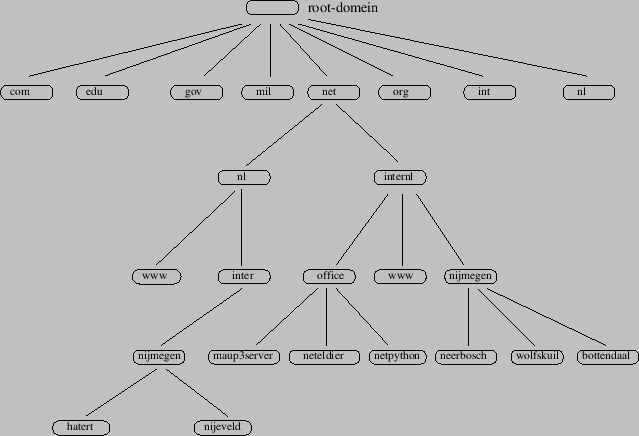
\includegraphics[width=7cm]{img/dnshierarchie.png}\\
\end{center}
\pause
{\bf domein}: 1 tak met alle bijbehordende vertakkingen. Bv. internl.net\\
\pause
{\bf zone}: hetzelfde zonder de {\it gedelegeerde} delen. Bv. internl.net zonder nijmegen.internl.net\\
Nameserver: verantwoordelijk voor zijn stukje (zone) van de boom.
\end{styleframe}

\section{Hoe werkt DNS?}
\subsection{client ({\it resolver}) en server ({\it nameserver})}
\begin{styleframe}
	\frametitle{client ({\it resolver}) en server ({\it nameserver})}
Hoe wordt het IP-adres behorende bij een naam gevonden?\\
~\\
DNS is client-server georienteerd:
\begin{description}[nameserverxx]
	\item[resolver] de client die de vraag stelt
	\item[nameserver] de server die het antwoord gaat geven
\end{description}
\end{styleframe}

\subsection{resolver}
\begin{styleframefrag}
	\frametitle{resolver 1/2}
\begin{itemize}
\item Wat is een resolver?\\
\pause
Veelal simpelweg een bibliotheek routine (functie gethostbyname()), ingebakken in client toepassingen als bv. firefox, thunderbird etc...\\
\pause
\item Hoe weet een resolver nu welke name-server te vragen?\\
	\begin{itemize}
	\item Configuratie in /etc/resolv.conf:\\
{\tt search internl.net nijmegen.internl.net\\
nameserver 202.219.13.156\\ 
nameserver 202.67.14.144}
\pause ({\bf IP adressen!})\\
\pause
	\item Op desktop-clients (bv. bij ubuntu) zie je:\\
{\tt nameserver 127.0.1.1\\
search localhost\\}
Dan wordt de vraag doorgegeven aan ''NetworkManager''\\
	\end{itemize}
\end{itemize}
\end{styleframefrag}

\begin{styleframefrag}
	\frametitle{resolver 2/2}
\begin{itemize}
\item Een resolver overhandigt altijd een FQDN ({\it Fully Qualified Domain Name}):
	\begin{itemize}
	\item Bij een enkele naam vult de resolver deze aan met het default domein.
	\item Indien de naam uit 2 of meer labels bestaat (dus in elk geval 1 punt bevat) wordt deze naam beeindigt met een punt. Levert dit niets op dan wordt alsnog de naam aangevuld met het default domein.
	\end{itemize}
\pause
\item {\bf Geen} goed idee om zelf de laatste punt toe te voegen..
\pause
\item {\bf Geen} goed idee om bv. een {\it toplevel} domainnaam te kiezen v\'o\'or een lager domein:\\
bv. {\tt www.org.internl.net}
\end{itemize}
\end{styleframefrag}

\subsection{nameserver}
\begin{styleframe}
	\frametitle{nameserver}
\begin{itemize}
	\item Werkpaard
	\item Verschil in functionaliteit tussen nameservers (straks meer)
	\item In tegenstelling tot een resolver gewoon zichtbaar: een daemon (veelal {\it named} (package {\it bind9} (ubuntu)))
\end{itemize}
\end{styleframe}

\subsection{een voorbeeld van de werking}
\begin{styleframefrag}
        \frametitle{een voorbeeld van de werking}
\begin{center}
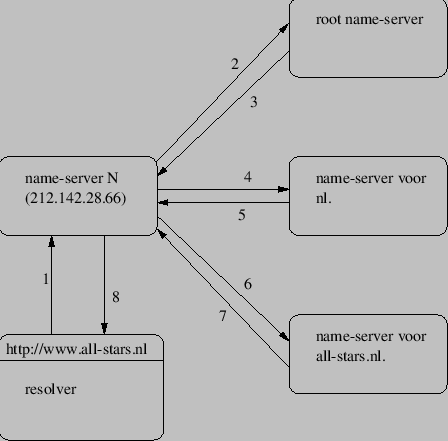
\includegraphics[width=5.6cm]{img/dns_voorbeeld.png}\\
\end{center}
\pause
Dit SCHREEUWT om het herinvoeren van HOSTS.TXT..
\pause
Maar:
\begin{itemize}
	\item[] Bovenstaand voorbeeld is een {\it worst case scenario}
	\item[] Praktijk: caching
\end{itemize}
\end{styleframefrag}

\subsection{caching nameservers}
\begin{styleframe}
        \frametitle{caching nameservers}
\begin{itemize}
	\item Vrijwel nergens {\it autoritair} voor: ze bevatten geen {\it zone-data}.
	\item Ook wel {\it recursive} nameservers genoemd.
	\item Veelal meer dan 1 geconfigged voor een client PC (DNS is belangrijk!!).
	\item Worden door je provider beschikbaar gesteld:\\
	 Geef je vaak op als ''DNS-servers'' in je netwerk-configuratie van je PC.
	\item Ook vrij te gebruiken caching nameservers: OpenDNS, Google Public DNS, ...
\end{itemize}
\end{styleframe}

\subsection{authoritative name-servers}
\begin{styleframe}
        \frametitle{authoritative name-servers}
\begin{itemize}
	\item Autoritair voor 1 of meerdere zones
	\item Veelal master met 1 of meerdere slaves
(vroeger ook wel primary master en secondary masters genoemd, alleen Microsoft houdt hardnekkig vast aan deze namen (nog steeds?))
	\item Meerdere servers: {\it redundancy}, spreiding drukte
	\item Administratie zonedata op 1 plek (master)
	\item Kunnen evt. ook recursie doen
\end{itemize}
\end{styleframe}

\section{De omgekeerde wereld}
\subsection{x.x.x.x.in-addr.arpa.}
\begin{styleframe}
        \frametitle{De omgekeerde wereld}
\begin{center}
''Reverse DNS'':\\
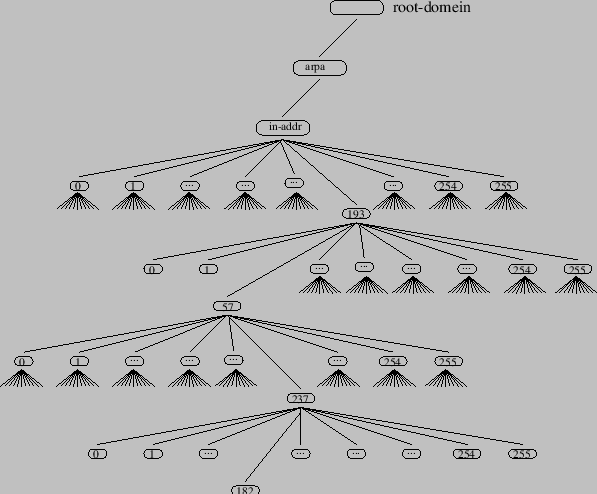
\includegraphics[width=5.6cm]{img/in-addr.png}\\
\end{center}
\pause
\begin{itemize}
	\item Elk domein heeft 256 subdomeinen
	\pause
	\item Op 1 na de grootste tak in de boom (alle IPv4 adressen)
	\pause
	\item Naam begint ook onderaan maar IP-adres formuleer je andersom (!)
	\pause
	\item Autoriteit voor DNS en reserve DNS kan prima verschillen (komt zelfs vaak voor)
\end{itemize}
\end{styleframe}

\section{Zonedata}
\subsection{Resource Records (RRs)}
\begin{styleframe}
        \frametitle{Resource Records (RRs)}
\begin{itemize}
        \item Een authoritative nameserver beheerd de data voor 1 of meer zones: de zonedata
        \item Zonedata bestaat uit gewone ASCII regels: de {\it resource records} (vaak aangeduid in de leteratuur als RRs).
	\pause
        \item Verschillende soorten resource records:
	\begin{itemize}
		\item SOA-record: Start Of Authority, administratieve data
		\item NS-records: de authoritative nameservers
		\item MX-records: wat zijn de mailservers voor dit domein?
		\item A-records: wat is het IP-adres (default, meest voorkomend)
		\item CNAME-records: wat is de {\bf echte} (Canonical) naam? 
		\item PTR-records: wat is de naam? (in *.addr.arpa. zones)
	\end{itemize}
\end{itemize}
\end{styleframe}

\subsection{Voorbeelden RR's}
\begin{styleframefrag}
        \frametitle{Voorbeelden RR's}
{\scriptsize
linuxnijmegen.nl.  86400  IN   SOA   ns1.am13.siteground.biz.  root.serv01.am13.siteground.biz. 2014112706 86400 7200 3600000 86400
~\\
~\\
\pause
linuxnijmegen.nl.       86400   IN      NS      ns1.am13.siteground.biz.\\
linuxnijmegen.nl.       86400   IN      NS      ns2.am13.siteground.biz.
~\\
~\\
\pause
linuxnijmegen.nl.       3600    IN      MX      30 mx30.mailspamprotection.com.\\
linuxnijmegen.nl.       3600    IN      MX      10 mx10.mailspamprotection.com.\\
linuxnijmegen.nl.       3600    IN      MX      20 mx20.mailspamprotection.com.
~\\
~\\
\pause
www.linuxnijmegen.nl.   14400    IN      CNAME   linuxnijmegen.nl.\\
linuxnijmegen.nl.       14400    IN      A       109.73.229.96
~\\
~\\
\pause
96.229.73.109.in-addr.arpa. 86400 IN    PTR     ip-109-73-229-96.siteground.com.
~\\
~\\
\pause
229.73.109.in-addr.arpa. 172800 IN      NS      ns1.clev1.net.\\
229.73.109.in-addr.arpa. 172800 IN      NS      ns2.clev1.net.
}
\end{styleframefrag}

\section{Tools}
\subsection{dig}
\begin{styleframe}
        \frametitle{dig 1/2}
Het commando {\it dig} is onderdeel van het package ''dnsutils'' (ubuntu)\\
~\\
\pause
Voorbeelden:\\
Wat is het IP-adres van www.linuxnijmegen.nl?
\pause
\begin{itemize}
	\item {\tt dig www.linuxnijmegen.nl}
\end{itemize}
~\\
\pause
Wat zijn de nameservers voor linuxnijmegen.nl?
\pause
\begin{itemize}
	\item {\tt dig ns linuxnijmegen.nl}
\end{itemize}
~\\
\pause
Wat zijn de mailservers voor linuxnijmegen.nl? Vraag het aan een authoritative nameserver.
\pause
\begin{itemize}
	\item {\scriptsize {\tt dig mx linuxnijmegen.nl @ns1.am13.siteground.biz}}
\end{itemize}
~\\
\pause
Wat is de naam van 109.73.229.96?
\pause
\begin{itemize}
	\item {\tt dig -x linuxnijmegen.nl}
\end{itemize}
\end{styleframe}

\begin{styleframe}
        \frametitle{dig 2/2}
Wat is het IPv6-adres van colo.all-stars.nl?
\pause
\begin{itemize}
	\item {\tt dig AAAA colo.all-stars.nl}
	\item[] (verwar niet met {\tt dig -6 colo.all-stars.nl} !)
\end{itemize}
~\\
\pause
{\footnotesize Wat is de naam van het IPv6-adres: 2a01:3a8:100:16:1:cafe:0:80?}
\pause
\begin{itemize}
	\item {\tt dig -x 2a01:3a8:100:16:1:cafe:0:80}
\end{itemize}
~\\
\pause
Gehele zone opvragen ({\it zone transfer}):
\pause
\begin{itemize}
	\item {\scriptsize {\tt dig axfr linuxnijmegen.nl @ns1.am13.siteground.biz}}
	\item[] Dit is bv. wat de slaves doen (en mogen).
\end{itemize}
~\\
\pause
Vermijd caching (alleen voor ''debug'' doeleinden): +trace
\pause
\begin{itemize}
	\item {\tt dig +trace +nodnssec linuxnijmegen.nl}
\end{itemize}
\end{styleframe}

\begin{styleframefrag}
        \frametitle{geoip}
{\footnotesize Onderstaande heeft niets met DNS te maken (maar is wel leuk :-))}
~\\
~\\
Een naam zegt niet altijd waar een host zich bevind.\\
Bv.: is de host die luistert naar {\tt www.linuxnijmegen.nl} in Nederland?\\
Kun je achterhalen met commando geoiplookup (package ''geoip-bin'' (ubuntu))
\begin{itemize}
	\item[] {\tt geoiplookup 109.73.229.96}
\end{itemize}
~\\
\pause
Ook leuk:
\begin{itemize}
	\item[] {\tt sudo traceroute -I www.triplej.com.au}
\end{itemize}
~\\
\pause
Nog leuker:
\scriptsize
\begin{verbatim}
sudo traceroute -I www.triplej.com.au | tail -n +2 | 
   sed 's/^.*(\(.*\)).*$/\1/'| grep -v '\*' |
   xargs -n1 geoiplookup | grep -v 'Address not found' |
   cut -d, -f2 | sed 's/^ //' | uniq -c
\end{verbatim}
\end{styleframefrag}

\section{Configuratie van bind}
\subsection{/etc/named.conf}
\begin{styleframefrag}
        \frametitle{Configuratie van bind}
\begin{itemize}
	\item {\it bind} meest gebruikte nameserver software
	\item Configfile veelal /etc/named.conf (meestal chrooted)
	\item Rest config veelal onder /var/named (meestal chrooted)
\end{itemize}
Voorbeeld inhoud file /etc/named.conf (heel summier) voor de authoritative nameserver voor kwalinux.nl:\\
{\scriptsize
\begin{verbatim}
options {
allow-query     { any; };
allow-transfer  { 188.142.103.98; 149.210.136.182;};
recursion no;
}
zone "." IN {
        type hint;
        file "named.ca";
};
include "/etc/named.rfc1912.zones";
// for which zones are we authoritative?
include "/etc/named.conf.master";
\end{verbatim}
}
\end{styleframefrag}

\subsection{config zones}
\begin{styleframefrag}
        \frametitle{/etc/named.conf.master}
{\small
\begin{verbatim}
zone "kwalinux.nl" {
        type master;
        file "/var/named/master/kwalinux.nl";
};
zone "linuversity.nl" {
        type master;
        file "/var/named/master/linuversity.nl";
};
zone "reisavonturen.net" {
        type master;
        file "/var/named/master/reisavonturen.net";
};
zone "travelstories.net" {
        type master;
        file "/var/named/master/travelstories.net";
};
\end{verbatim}
}
\end{styleframefrag}

\subsection{inhoud zonefile voor kwalinux.nl (zonedata voor kwalinux.nl)}
\begin{styleframefrag}
        \frametitle{/var/named/master/kwalinux.nl}
{\tiny
\begin{verbatim}
@           IN      SOA     auth1.dns.kwalinux.nl. hostmaster.kwalinux.nl. (
                            30              ; serial
                            6H              ; refresh
                            30M             ; retry
                            1d            ; expiry
                            1H )            ; minimum


@           IN      NS      auth1.dns.kwalinux.nl.
@           IN      NS      auth2.dns.kwalinux.nl.

@           IN      A       78.31.117.114
@           IN      AAAA    2001:7b8:634:4100:20c:29ff:feb4:fce2

@           IN      MX      0 mail.kwalinux.nl.
@           IN      TXT     "v=spf1 mx a ~all"

localhost   IN      A       127.0.0.1

auth1.dns   IN      A       78.31.117.114
auth1.dns   IN      AAAA    2001:7b8:634:4100:20c:29ff:feb4:fce2
auth2.dns   IN      A       188.142.103.98
mail        IN      A       78.31.117.114
www         IN      A       78.31.117.114
www         IN      AAAA    2001:7b8:634:4100:20c:29ff:feb4:fce2
ww6         IN      AAAA    2001:7b8:634:4100:20c:29ff:feb4:fce2
doc         IN      A       78.31.117.114
m           IN      A       78.31.117.114
\end{verbatim}
}
\end{styleframefrag}

\subsection{Gevorderde technieken}
\begin{styleframe}
        \frametitle{gevorderde technieken}
\begin{itemize}
	\item {\it dynamic updates}. Vooral handig bij het gebruik van IP-adressen verkregen met DHCP voor hosts met vaste hostnamen.
	\pause
	\item {\it incremental zone transfers}. Alleen de zone-data die gewijzigd is wordt opgehaald door de slaves.
	\pause
	\item Secure DNS (DNSSEC): zekerheid gewenst dat de verkregen DNS informatie ook werkelijk de juiste is.\\
	\pause
Heikele punten m.b.t. DNSSEC:
	\begin{itemize}
		\item Extra resource records nodig, o.a.:
		\begin{itemize}
			\item SIG-record. Dit record bevat een cryptografische {\it signature} voor resource records.
			\item KEY-record. Dit is een record met public keys van SIG-records.
		\end{itemize}
		\pause
		\item Meer complexiteit: bijhouden van DNS niet meer ''met de hand'' maar met tooling.
		\pause
		\item De performance van DNSSEC laat nog te wensen over.
	\end{itemize}
\end{itemize}
\end{styleframe}

\section{Vragen en antwoorden}
\begin{styleframe}
        \frametitle{vragen en antwoorden}
Eerst een {\bf Tip:} Sluit netwerk-issues uit door eerst met IP-adressen te werken.
\pause
{\scriptsize
\begin{description}[Q]
	\item[Q] ''We willen ons domein graag verhuizen maar blijft onze mailserver dan bereikbaar?''
	\pause
	\item[A] ''Geen probleem. Zolang de zonedata gewoon meeverhuisd wordt.''
	\pause
	\item[Q] ''We willen het IP-adres van onze webserver veranderen. Hoelang duurt het dan voordat alle name-servers het nieuwe IP-adres weten?''
	\pause
	\item[A] ''Wanneer geen\'e\'en caching nameserver de oude data nog in de cache heeft. Check voor jezelf met dig ''naam webstite''.
	\pause
	\item[Q] ''Wij hebben een eigen mail-server maar we ontvangen geen mail!''
	\pause
	\item[A] ''Check de MX records voor het domein.''
	\pause
	\item[Q] ''Ik kan pingen naar de ftp-server maar zodra ik ernaar probeer te ftp-en wordt de verbinding direct verbroken?''
	\pause
	\item[A] ''Waarschijnlijk gaat de reverse lookup van je eigen IP-adres fout: sommige ftp daemons willen dat.''
	\pause
	\item[Q] ''Ik wil mijn nieuw gemaakte website testen met de echte url, kan dat zomaar?''
	\pause
	\item[A] ''Edit op je client je eigen hosts-file (/etc/hosts).''
	\pause
	\item[Q] ''Ik heb geen internet!''
	\pause
	\item[A] ''Als pingen naar IP-adressen wel werkt: misschien heeft je provider een probleem.. (zelden)''
	\pause
	\item[Q] ''Waarom zijn er maar 13 root nameservers?''
	\pause
	\item[A] ''Meer past(te) er niet in een UDP pakket. Overigens zijn er dankzij {\it anycast} veel meer dan 13.''
\end{description}
}
\end{styleframe}

